\documentclass[a4paper]{article}
\usepackage{amsmath}
\usepackage[english,dutch]{babel}
\usepackage[fixlanguage]{babelbib}
\usepackage{booktabs}
\usepackage{dcolumn}
\usepackage{graphicx}
\usepackage{hyperref}

\selectbiblanguage{dutch}

\author{Pieter Belmans}
\title{Opgave tweede les}

\begin{document}
\maketitle

\begin{abstract}
  Probeer dit document na te maken, zoals vorige keer zijn er geen speciale dingen gebruikt: enkel materie die we deze les gezien hebben of dingen die snel op te zoeken zijn. Als een moeilijke wiskunde uitdrukking je niet lukt\footnote{Sorry, ik vond geen zinniger onderwerp voor een tabel\ldots}, geen probleem, dat zien we volgende les pas.
\end{abstract}

\tableofcontents

\section{Tabellen}
In Tabel~\ref{table:transcendental-numbers} geef ik een overzicht van enkele transcendente getallen, dit op basis van~\cite{wiki:transcendental-number}. Voor zij die het nog niet zouden weten,~$\pi$ schrijf je als~\verb|$\pi$| en~$e$ als~\verb|$e$|. Dat al deze getallen transcendent zijn is een gevolg van de stelling van~Lindemann--Weierstrass.

\begin{table}[h!]
  \centering
  \begin{tabular}{cp{.5\textwidth}D{.}{.}{-1}}
    \toprule
    symbool & oorsprong & \multicolumn{1}{c}{decimale voorstelling} \\\midrule
    $\pi$ & de cirkel & 3.14159265\ldots \\
    $e$ & Exponenti\"ele processen zoals deze wel vaker in de natuur voorkomen, biologen kennen dit bijvoorbeeld voor populatieaanwas. Fysici zullen dit eerder kennen uit fissieprocessen. \newline Economen daarentegen kennen het getal vooral via inflatie. & 2.71828\ldots \\
    $\tan\left( \frac{11\sqrt{2}}{10} \right)$ & mijn zieke geest & 65.952\ldots \\
    \bottomrule
  \end{tabular}
  \caption{Een overzicht van transcendente getallen}
  \label{table:transcendental-numbers}
\end{table}

\section{Afbeeldingen}
Zoek je favoriete afbeelding van een kat (of als je echt wil, deze kat) en voeg deze toe. In Figuren~\ref{figure:cat} en~\ref{figure:cat-2} wordt dus mijn keuze gegeven, telkens met een bepaalde placement modifier.

\begin{figure}[t]
  \centering
  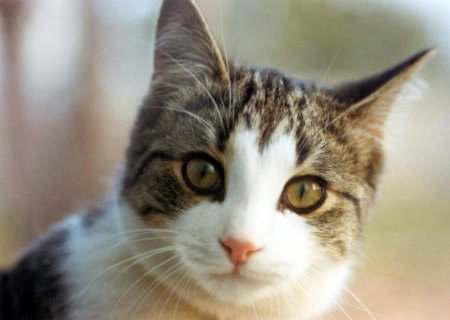
\includegraphics[height=4cm]{cat.jpg}
  \caption{Een kat}
  \label{figure:cat}
\end{figure}

\begin{figure}[b]
  \centering
  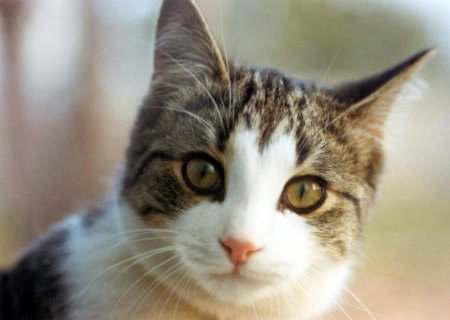
\includegraphics[height=3cm]{cat.jpg}
  \caption{Een kat}
  \label{figure:cat-2}
\end{figure}

\section{Geschiedenis}
Als je wil weten hoe~\TeX\ in elkaar zit verwijs ik je graag door naar~\cite{texbook}.

\bibliographystyle{babalpha}
\bibliography{opgave-2}
\end{document}
